\documentclass[a4paper]{article}
%Gummi|061|=)
\usepackage{amsmath}
\usepackage{amsthm}
\usepackage{amsbsy}
\usepackage{amssymb}
\usepackage{inputenc}
\usepackage{graphicx}
\usepackage{siunitx}
\usepackage{selinput}
\usepackage{booktabs}
\SelectInputMappings{%
adieresis={ä},
germandbls={ß},
}
\title{\textbf{V53: Mikrowellen}}
\author{Martin Bieker - martin.bieker@udo.edu\\
Julian Surmann - julian.surmann@udo.edu\\
\\
Durchgef\"{u}hrt am 20.04.2015\\
TU Dortmund}
\date{}
\usepackage{graphicx}
\begin{document}
\renewcommand\tablename{Tabelle}
\renewcommand\figurename{Abbildung}
\maketitle
\thispagestyle{empty}
\newpage
\clearpage
\setcounter{page}{1}
\section{Einleitung}
In diesem Versuch werden die Eigenschaften von Mikrowellen in einem rechteckigen Hohlleiter untersucht.

\section{Theorie}
Durch einen Hohlleiter kann Energie in Form von elektromagnetischen Wellen übertragen werden. Die Wellen kommen in verschiedenen Moden vor, jede hat eine eigene elektrische und magnetische Feldverteilung. Je nach Ausrichtung der Felder handelt es sich um transversal elektrische oder transversal magnetische Moden, abhängig davon, welche Feldkomponente senkrecht zur Ausbreitungsrichtung der Welle ist. Die Feldstärke ist im Zentrum des Querschnittes am größten.

\subsection{Das Reflex-Klystron}
\begin{figure}[h]
\centering
\includegraphics[scale=0.7]{klystron.png}
\caption{Schematischer Aufbau eines Reflex-Klystrons $[1]$}
\label{klystron}
\end{figure}

\noindent
In diesem Versuch werden die Mikrowellen mit einem Reflex-Klystron (Abbildung \ref{klystron}) und einer Gunndiode erzeugt. Im Reflexklystron werden Elektronen aus einer erhitzten Kathode gelöst und von zwei Beschleunigungsgittern beschleunigt. Nach passieren der Gitter werden die Elektronen von einem negativ geladenen Reflektor abgebremst und die Bewegungsrichtung der Elektronen umgekehrt. Bei dem Bereich zwischen den Gittern handelt es sich um die Resonatorkammer, in der die Elektronen durch Influenz ein schwaches elektromagnetisches Feld erzeugen. Wenn das Klystron schwingt, werden die Elektronen während des Aufenthalts in der Resonatorkammer entweder beschleunigt oder abgebremst, sodass sie verschiedene Umkehrpunkte besitzen und anschliessend gebündelt auftreten. Dies wird als Geschwindigkeitsmodulation bezeichnet. Werden die Bündel im Resonator abgebremst, geben sie Energie an den Resonator ab, er schwingt.

\noindent
Die Frequenz der Klystronschwingung kann mit Hilfe der mechanischen und elektronischen Abstimmung eingestellt werden. Bei der mechanischen Abstimmung wird das Volumen des Resonators verändert. Eine leichte Änderung der Resonatorfrequenz kann auch durch eine Änderung der Resonator- bzw Reflektorspannung erreicht werden, die wird elektronische Abstimmung genannt.

\noindent
Um die Ausgangsleistung mit einem selektiven Verstärker zu bestimmen, wird das Signal zusätzlich amplitudenmoduliert, z.B. mit einer Rechteck- oder Sinusspannung.

\section{Aufbau}
\begin{figure}[h]
\centering
\includegraphics[scale=1.0]{aufbau1.png}
\caption{Schaltung zur Messung der Zeitabhängigkeit der Amplitude $[1]$}
\label{S1}
\end{figure}
Der grundlegende Aufbau (Abbildung XXX) wird bei allen Versuchsteilen benötigt. Er besteht aus dem Klystron-Oszillator mit Speisegerät, einem Ferrit-Isolator, einem Frequenzmesser und einem Dämpungsglied.
ABBILDUNG
Die Mikrowellen werden im Klystron in einem ersten Teilstück des Hohlleiters erzeugt. Am Klystron wird der Ferrit-Isolator angeschlossen. Dieser unterdrückt Mikrowellenstrahlung im Hohlleiter, die sich in Richtung des Klystrons bewegt, um dieses nicht zu beeinflussen. Im Anschluss an den Isolator wird der Frequenzmesser eingesetzt. Dieser besteht aus einem koaxialen Resonator, dessen Resonanzfrequenz auf \SI{100}{\hertz} genau eingestellt werden kann. Falls es sich bei der eingestellten Resonanzfrequenz um die Klystronfrequenz handelt, ist ein Minimum (ein sog. dip) bei der am Ende abgegriffenen Leistung zu erkennen. An den Frequenzmesser wird das einstellbare Dämpfungsglied angeschlossen. Hierbei handelt es sich um einen geeichten Folienabschwächer, der mit Hilfe einer Mikrometerschraube auf einen Dämpfungsgrad eingestellt werden kann. Dazu ist auf dem Dämpfungsglied eine Eichkurve angebracht, an der man die Dämpfung in \SI{}{\decibel} in Abhängigkeit von der Einstellung der Mikrometerschraube ablesen kann.

\noindent
Im Anschluss an das Dämpfungsglied werden die versuchsspezifischen Bauteile angebracht, die im folgenden erläutert werden.
\paragraph{Stehwellendetektor}
Der Stehwellendetektor besteht aus einer Sonde, die sich durch einen Schlitz im Hohlleiter in Längsrichtung und in der Tiefe verstellen lässt. An der Sonde ist eine Detektordiode angebracht, deren gleichgerichtetes Signal an eine BNC-Buchse geführt wird.
\paragraph{Gleitschraubentransformator}
Der Gleitschraubentransformator wird verwendet, um einen fehlangepassten Kreis zu korrigieren. Er besteht aus einem als Blindwiderstand wirkenden Stift, der wie die Sonde beim Stehwellendetektor bewegt werden kann.
\paragraph{Einstellbarer Kurzschluss} Mit diesem Bauteil lassen sich Reflexionen mit genau definierter Phasenlage einstellen. Dazu ist die Rückwand des Hohlleiters als einstellbare Präzisionsschraube ausgeführt.
\paragraph{Abschluss} Der Abschluss besteht aus einem Hohlleiter, der so mit einem Absorbermaterial gefüllst ist, dass fast die gesamte Leistung absorbiert wird.
\paragraph{Detektor} Der Detektor besteht aus einem Hohlleiter-Endstück und einer Diode, die an eine BNC-Buchse angeschlossen ist.
\paragraph{Messgeräte} Um die an den BNC-Buchsen abgegriffene Leistung zu messen, werden ein Oszilloskop und ein SWR-Meter benutzt. Beim SWR-Meter (standing-wave-ratiometer) handelt es sich um einen selektiven \SI{1000}{\hertz}-Verstärker mit kleinem Rauschen. Es hat zwei Skalen, um die Leistung abzulesen: Die VSWR-Skala (voltage-standing-waveratio) und die \SI{}{\decibel}-Skala.


\section{Durchführung und Auswertung}
\subsection{Erstellung eines Modendiagramms}
Im ersten Teilversuch soll der Verlauf der abgestrahlten Mikrowellenleistung in Abhängigkeit von der angelegten Reflektorspannung untersucht werden.
Hierzu wird das Klystron mit einer \SI{50}{\hertz}-Sinusspanunung moduliert.
Dann wird die Reflektorspannung am Speisegerät auf etwa \SI{200}{\volt} eingestellt.
Mit dem Frequenzmesser wird die Mittenfrequenz 
\[
f_0 = \SI{9038,4}{\mega\hertz}
\]
des Modus bestimmt, in dem dieser durchgestimmt wird bis ein Dip auf der Spitze der Modenkurve zu sehen ist (vgl Abb. \ref{dip}).
\begin{figure}[h]
\centering
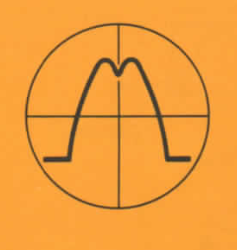
\includegraphics[scale=0.7]{mode_dip.png}
\label{dip}
\caption{Diese Abbildung zeigt die Position des Dips des Frequenzmessers zur Bestimmung der Mittenfrequenz eines Modus.[1]}
\end{figure}
Das Klystron wird mit Hilfe des Abstimmknopfs auf eine Frequenz von
\[
\SI{9000}{\mega\hertz} 
\]
abgestimmt. Am Oszilloskop wird die Amplitude des Modus und wie oben beschrieben die Frequmz der Modenspitze bestimmt.
Des Weiteren wird am Klystron-Speisegerät die Reflektorspannung abgelesen. Danach wird die Reflektorspannung einmal erhöht und einmal verringert, 
bis der Rand der Modenkurve in der Mitte des Oszillogramms liegt. 
Diese Spannungen sind die obere und untere Schwingungseinsatz-Spannung.
Anschließend wird die Reflektorspannung schrittwgeise gesenkt und die voherigen Messungen für zwei weitere Moden wiederholt.
Die Ergebnisse befinden sich in Tabelle \ref{modedata}.
\begin{table}[h]
\centering
\begin{tabular}{rccc}
\toprule
& 1. Modus & 2. Modus & 3. Modus \\
\midrule
$V_0$ in \si{\volt}  & 218 & 140 & 72 \\
$V_1$ in \si{\volt} & 201 & 120 & 68 \\
$V_2$ in \si{\volt} &232.5 & 151 & 92 \\
$A_0$ in div & 6.7 & 6.7 & 5.3 \\
$f_0$ in \si{\mega\hertz} & 9000 & 9004 & 9010 \\
\bottomrule
\end{tabular}
\label{modedata}
\caption{Diese Tabelle enthält die gemessene Mikrowellenleistung in Abhängigkeit von der Reflektorspannung für drei Moden des Klystrons}
\end{table}

\noindent
In Abbildung \ref{modeplot} sind die gemessenen Werte der drei Moden nocheinmal graphisch dargestellt.

\begin{figure}[h]
\centering
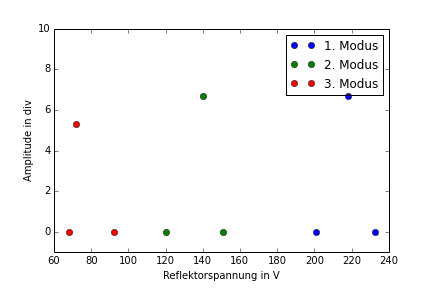
\includegraphics[scale = 0.7]{mode_plot.png}
\caption{Diese Abbildung zeigt für drei Moden des Klystrons die gemessene Leistung in Abhängigkeit von der Reflektorspannung}
\label{modeplot}
\end{figure}



\subsection{Elektronische Abstimmung}
In diesem Teilversuch soll die elektronische Bandbreite $\Delta f$ und die Abstimm-Empfindlichkeit des Klystrons bestimmt werden.
Hierzu wird das Klystron auf eine Frequenz von \SI{9000}{\mega\hertz} abgestimmt. 
Die Reflektorspannung wird jeweils erhöht und gesenkt bis sich die Punkte halber Leistung in der Mitte des Oszillogramms befinden.
Der Frequenzmesser wird durchgestimmt bis sich der Dip ebenfalls auf der Mittellinie des Oszillokops liegt. 
Die auf diese Weise ermittelten Spannungen und Frequenzen betragen:
\begin{itemize}
\item $f = \SI{9000}{\mega\hertz}$
\item $V = \SI{218}{\volt}$
\item $f' = \SI{9025}{\mega\hertz}$
\item $V' = \SI{225}{\volt}$
\item $f'' = \SI{8973}{\mega\hertz}$
\item $V'' = \SI{202,5}{\volt}$
\end{itemize}
Die elektronische Bandbreite beträgt
\[
\Delta f = \SI{52}{\mega\hertz}
\]
und die Abstimm-Empfindlichkeit:
\[
\frac{f' - f''}{V' - V''} = \SI{2,3}{\mega\hertz\per\volt}.
\]
\subsection{Frequenzmessung}
In diesem Versuchsteil soll die Frequenz des Reflexklystrons aus der Wellenlänge einer stehenden Welle bestimmt werden. Dazu wird zunächst die Sonde des Stehwellendetektors in die Mitte des Hohlleiters abgesenkt. Das Klystron wird mit einer \SI{1}{\kilo\hertz} Rechteckspannung moduliert und mit einer Reflektorspannung von ca. \SI{200}{\volt} betrieben. Als Erstes wird die Frequenz des Klystrons mit Hilfe des Frequenzmessers bestimmt. Hierzu wird der Frequenzmesser durchgestimmt bis am SWR-Meter ein verringertes Signal (Dip) gemessen wird. Die gemessene Frequenz beträgt
\[
f_{mess} =  \SI{9000}{\mega\hertz}.
\]

\noindent
Damit sich im Hohlleiter eine stehende Welle bildet, muss der Abschluss am Ende des Messaufbaus durch einen Kurzschluss ersetzt werden. Jetzt wird mit der Sonde des Stehwellen-Detektors die Position zweier benachbarter Minima bestimmt:

\begin{itemize}
\item $x_1 = \SI{89.1}{\milli\meter}$
\item $x_2 = \SI{118.95}{\milli\meter}$
 \end{itemize}
Die Wellenlänge der Mikrowellen im Hohlleiter ergibt sich als das Doppelte des Abstands dieser Punkte.
\[
\lambda = \SI{59,7}{\milli\meter}
\]

\noindent
Des Weiteren wird die geometrische Abmessung $a$ des Wellenleiters bestimmt:
\[
a = \SI{22,85}{\milli\meter}
\]
Aus diesen Werten kann die Frequenz $f$ der Mikrowellen berechnet werden:
\[
f = c \cdot \sqrt{\left(\frac1\lambda\right)^2+ \left(\frac1{2a}\right)^2} = \SI{8319}{\mega\hertz}.
\]
\subsection{Dämpfungsmessung}
Zur Messung der Dämpfung darf sich keine stehende Welle im Wellenleiter befinden.
Daher wird der einstellbare Kurzschluss durch einen Abschluss ersetzt, da dieses Bauteil die einfallenden Mikrowellen fast vollständig absorbiert. Am SWR-Meter wird der Verstärker so eingestellt, dass dieses als Referenzwert \SI{0}{\dB} anzeigt.
Die Dämpfung wird am Dämpfungsglied eingestellt, indem die Mikrometerschraube um eine Strecke $\Delta x$ in den Hohlleiter eingeschoben wird.
$\Delta x$ wird in \SI{2}{\milli\meter}-Schritten erhöht und die resultierende Dämpfung mit dem SWR-Meter bestimmt.
Des weiteren wurde zu den jeweiligen Werten von $\Delta x$ ein Wert für die Dämpfung aus der Eichkurve des Dämpfungsglieds abgelesen.
Diese Werte sind in Tabelle \ref{daempftab} aufgeführt und in Abbildung \ref{daempf_plot} graphisch dargestellt.

\begin{table}[h]
\centering
\begin{tabular}{ccc}
\toprule
SWR-Meter Ausschlag in \si{\dB}  & $\Delta x$ in \si{\milli\meter}  & Dämpfung aus der Eichkurve in \si{\dB} \\
\midrule
0 & 0.00 & 0 \\
2 & 1.85 & 6 \\
4 & 2.32 & 10 \\
6 & 2.59 & 13 \\
8 & 2.77 & 14 \\
10 & 2.99 & 17 \\
\bottomrule
\end{tabular}
\label{daempftab}
\caption{Diese Tabelle enthält die Ergebnisse der Dämpfungsmessung.}
\end{table}

\begin{figure}[h]
\centering
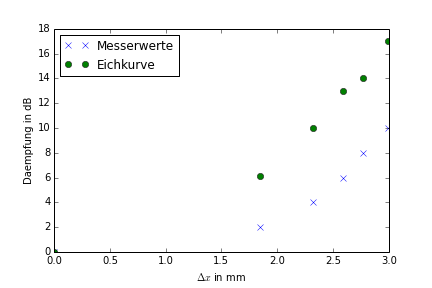
\includegraphics[scale=0.7]{daempf_plot.png}
\caption{Diese Abbildung zeigt die Dämpfung in Abbhängigkeit von der Position der Mikrometerschraube.}
\label{daempf_plot}
\end{figure}

\subsection{Bestimmung des SWR mit dem SWR-Meter}
In den letzten Teilversuchen soll das Spannungs-Stehwellenverhältnis (SWR) auf 3 verschiedene Arten bestimmt werden.
Das Klystron wird für diese Messung bei einer Frequenz von \SI{9}{\giga\hertz} betrieben und mit einer \SI{1}{\kilo\hertz}-Rechteckspannung moduliert. 
Als erstes wird das SWR direkt mit einem geigneten Messgerät (SWR-Meter) gemessen.
Dazu wird die Sonde des  Gleitschraubentransformators in die Mitte des Wellenleiters eingeführt und danach entlang der Messleitung verschoben. 
Es sind keine größeren Änderungen des Ausschlags des SWR-Meters zu beobachten.
Das liegt daran, dass sich im Hohlleiter auf Grund des Abschlusses am Ende des Messaufbaus keine stehende Welle bilden kann.
Nun soll das SWR in Abhängigkeit von der Sondentiefe bestimmt werden. Dazu wird die Tiefe der Sonde in \SI{2}{\milli\meter}-Schritten von \SI{3}{\milli\meter} auf \SI{9}{\milli\meter} erhöht.
Um die Anzeige des SWR-Meters zu normieren, wird die Sonde entlang des Hohlleiters verschoben, bis ein maximaler Ausschlag angezeigt wird. 
Die Verstärkung des Messgeräts wird so angepasst, dass dieses ein SWR von  \num{1,0} zeigt.
Dann wird die Sonde wieder in ein Minimum verschoben.
Der nun auf der Skala ablesbare Wert ist das zu messende Spannungs-Stehwellen Verhältnis.
Die auf diese Weise gewonnenen Daten sind in Tabelle \ref{swrtab} dargestellt.
\begin{table}
\centering
\begin{tabular}{cc}
\toprule
Sondentiefe in \si{\milli\meter} & SWR\\
\midrule
3 & 1.1 \\
5 & 1.2 \\
7 & 2.1 \\
9 & $\infty$\\
\bottomrule
\end{tabular}
\caption{Diese Tabelle zeigt das mit dem SWR-Meter gemessene Spannungs-Stehwellenverhältnis in Abhängigkeit von der Sondentiefe}
\label{swrtab}
\end{table}

\subsection{Bestimmung des SWR mit der "Abschwächer-Methode"}
In diesem Versuchsteil wird das SWR bei einer Sondentiefe von \SI{9}{\milli\meter} mit der so genannten Abschwächer-Methode bestimmt.
Dazu wird die Sonde zunächst wieder horizontal in ein Minimum verschoben und das Dämpfungsglied wird auf einen Wert von
\[
A_1 = \SI{20}{\dB}
\]
eingestellt. Die Verstärkung am SWR-Meter wird angepasst, damit dass Messgerät eine Intensität von \SI{3}{\dB} anzeigt. 
Nun wird das die Sonde entlang der Messleitung verschoben bis sich ein maximaler Ausschlag am SWR-Meter ergibt.
Dabei wird die Dämpfung schrittweise erhöht, so dass die gemessene Intensität stets \SI{3}{\dB} beträgt.
Die hierfür nötige Dämfung beträgt
\[
A_2 = \SI{4.3}{\dB}
\]
Mit dem folgenden Zusammenhang kann nun das SWR berechnet werden:
\[
S = 10 \cdot \frac{A_1 - A_2}{A_1} = \num{7,85}.
\]
\subsection{Bestimmung des SWR mit der "3\,dB-Methode"}
Abschließend soll das SWR bei gleicher Sondentiefe von \SI{9}{\milli\meter} mit der \SI{3}{\dB}-Methode bestimmt werden.
Zu Beginn wird die Sonde des Gleitschraubentransformators in ein Minimum verschoben und die Vertärkung am SWR-Meter angepasst, dass eine Intensität von
\SI{3}{\dB} registriert wird. 
Die Sonde wird nun nach links und nach rechts verschoben bis jeweils eine Intensität von \SI{0}{\dB} gemessen wird.
Diese Stellen liegen bei:
\begin{itemize}
\item $d_1 = \SI{88,1}{\milli\meter}$
\item $d_2 = \SI{86,4}{\milli\meter}$
\end{itemize}
Um das Spannungs-Stehwellenverhältnis zu berechnen wird auch die Hohlleiterwellenlänge $\lambda_g$ benötigt. 
Zur Bestimmung dieses Wertes wird der Abschluss am Ende der Messaparatur durch einen Kurzschluss ersetzt, damit sich im Hohlleiter eine stehende Welle
bildet.
Durch Verschieben der Sonde des Gleitschraubentransformators wird der Abstand zweier benachbarter Knoten (Minima) der stehenden Welle bestimmt.
\[
\lambda_g = \SI{50,4}{\milli\meter}.
\]
Aus diesen Werten ergibt sich durch den folgenden Zusammenhang das SWR:
\[
S = \sqrt{1 + \frac1{\sin^2 \frac{\pi \left( d_1-d_2\right)}{\lambda_g}}} = \num{9,5}.
\]


\section{Diskussion}

\end{document}

